% Todo:
% Change all the variables such that they are not in italics

\documentclass[12pt]{report}
\usepackage[a4paper]{geometry}
\usepackage[myheadings]{fullpage}
\usepackage{amsmath}
\usepackage{fancyhdr}
\usepackage{lastpage}
\usepackage{graphicx, wrapfig, setspace, booktabs}
% \usepackage[T1]{fontenc}
\usepackage[font=small, labelfont=bf]{caption}
\usepackage{fourier}
\usepackage[protrusion=true, expansion=true]{microtype}
\usepackage[english]{babel}
\usepackage{sectsty}
\usepackage{url, lipsum}
\usepackage{siunitx}
\usepackage{subcaption}
\usepackage[space]{grffile}
\usepackage[toc, page]{appendix}
\usepackage{braket}
\usepackage{xr}
\usepackage{gensymb}
\usepackage{floatrow}
\usepackage{bm}
\usepackage[section]{placeins}
\DeclareMathAlphabet{\mathpzc}{OT1}{pzc}{m}{it}

\externaldocument[RES-]{Chapters/DRIE.tex}
\externaldocument[A-]{Chapters/appendix.tex}
\sisetup{range-phrase = --, range-units = single}
\DeclareSIUnit\dBm{dBm}

% Resonator and noise chapter commands
\newcommand*\chem[1]{\ensuremath{\mathrm{#1}}}
% This command adds optionality of units at right side of equation
\makeatletter
\providecommand\add@text{}
\newcommand\tagaddtext[1]{%
  \gdef\add@text{#1\gdef\add@text{}}}%
\renewcommand\tagform@[1]{%
  \maketag@@@{\llap{\add@text\quad}(\ignorespaces#1\unskip\@@italiccorr)}%
}
\makeatother

% Muxmon chapter commands
\newcommand{\SIm}[2] {\text{\ensuremath{\SI{#1}{#2}}}}
\newcommand{\Ec}{E_\text{c}}
\newcommand{\Ej}{E_\text{J}}
\newcommand{\fbare}{f_\text{bare}}
\newcommand{\wbare}{\omega_\text{bare}}
\newcommand{\fres}{f_\text{r}}
\newcommand{\wres}{\omega_\text{r}}
\newcommand{\fqub}{f_\text{q}}
\newcommand{\wqub}{\omega_\text{q}}
\newcommand{\wdrive}{\omega_\text{d}}

\newcommand{\HRule}[1]{\rule{\linewidth}{#1}}
\newcommand{\figureinset}[3]{\llap{\parbox[b]{#2in}{#1\\\rule{0ex}{#3in}}}}

% \onehalfspacing
\setcounter{secnumdepth}{5}
\setcounter{tocdepth}{5}

%-------------------------------------------------------------------------------
% HEADER & FOOTER
%-------------------------------------------------------------------------------
\pagestyle{fancy}
\fancyhf{}
\setlength\headheight{15pt}
\fancyhead[L]{Serwan Asaad}
\fancyhead[R]{Delft University of Technology}
\fancyfoot[R]{Page \thepage\ of \pageref{LastPage}}
%-------------------------------------------------------------------------------
% TITLE PAGE
%-------------------------------------------------------------------------------

\begin{document}
\begin{titlepage}
\begin{center}
~\\ [4.0 cm]
\textsc{\LARGE Delft University of Technology}
\\ [3.0 cm]
\textsc{\Large Master Thesis}
\HRule{0.5 pt} \\
\LARGE \textbf{\uppercase{Master thesis}}
\HRule{2 pt} \\ [0.5 cm]

% Author and supervisor
\noindent
\begin{minipage}{0.4\textwidth}
\begin{flushleft} \large
\emph{Author:}\\
Serwan Asaad
\end{flushleft}
\end{minipage}%
\begin{minipage}{0.4\textwidth}
\begin{flushright} \large
\emph{Supervisors:} \\
Dr.~Alessandro Bruno \\
Christian Dickel
\end{flushright}
\end{minipage}
\\ [3.0 cm]
{\large \today}
\end{center}

\end{titlepage}


\author{
    Serwan Asaad
    Student ID: 4323475 \\
    Delft University of Technology \\
    Kavli Institute of Nanoscience\\
    Quantum Nanoscience Department\\
    Quantum Transport Group\\
    DiCarlo Lab}

\tableofcontents
\newpage

%-------------------------------------------------------------------------------
% Section title formatting
\sectionfont{\scshape}
%-------------------------------------------------------------------------------

%-------------------------------------------------------------------------------
% BODY
%-------------------------------------------------------------------------------

% \section*{Introduction}


\textbf{TODO:}
\begin{itemize}
  \item Explain heterodyne detection
  \item Explain VNA
  \item Explain that resonance frequency $\fres$ is not necessarily at the transmission minimum when the resonator exhibits asymmetry.
\end{itemize}



%!TEX root = ../thesis.tex
\label{part:DRIE}







% \part{asdf}{dfgs}
\part{Deep-reactive ion etched resonators\protect\blfootnote{This experiment has been published in Applied Physics Letters \textbf{106} 18 (2015).}}
\label{chapter:Resonators}

\chapter{Theory}
  \label{ch:theory}

  \section{Coplanar waveguide}
    \captionsetup[subfigure]{position=top}
    \begin{figure}[h]
      \begin{subfigure}{.49\textwidth}
        \begin{center}
            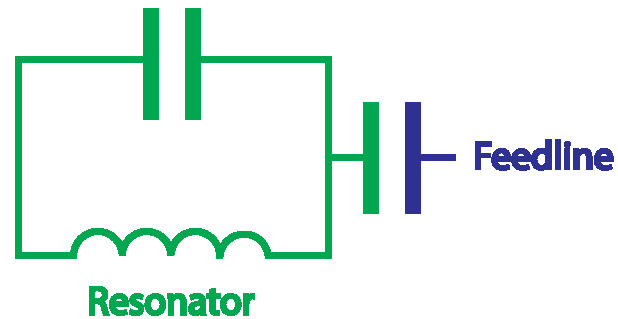
\includegraphics[width=.8\textwidth]{Figures/DRIE/resonator schematic joined.jpg}
        \end{center}
        \caption{ }
        \label{fig:CPW schematic}
      \end{subfigure}
      ~
      \begin{subfigure}{.49\textwidth}
        \begin{center}
            \includegraphics[width=.8\textwidth]{Figures/DRIE/CPW.png}
        \end{center}
        \caption{ }
        \label{fig:CPW intersection}
      \end{subfigure}
      \caption{\textbf{(a)} A resonator circuit diagram, including capacitive coupling to a feedline. \textbf{(b)} Cross-section on a CPW resonator. For a typical resonator $w=\SIm{12}{\micro \meter}$, $s=\SIm{5}{\micro \meter}$, $t=\SIm{200}{\nano \meter}$, and $h=\SIm{525}{\micro \meter}$.}
      \label{fig:CPW}
    \end{figure}
    \captionsetup[subfigure]{position=top}

    % \begin{wrapfigure}{r}{0.4\textwidth}
    %     \begin{center}
    %         \includegraphics[width=\textwidth]{Figures/DRIE/CPW.png}
    %     \end{center}
    %     \caption{Schematic of a coplanar waveguide. For a typical resonator $w=\SIm{12}{\micro \meter}$, $s=\SIm{5}{\micro \meter}$, $t=\SIm{200}{\nano \meter}$, and $h=\SIm{525}{\micro \meter}$.}
    %     \label{fig:CPW}
    % \end{wrapfigure}

    Superconducting coplanar waveguides (CPW) microwave resonators have versatile applications. They are used in single-photon detectors~\cite{tanner2010enhanced}, quantum-limited Josephson parametric amplifiers~\cite{castellanos2008amplification}, and in the context of circuit QED are used for memory storage, readout, and as interconnects. Coplanar waveguides consist of a long central conducting strip, with on both sides a neighbouring ground. The center conductor of width $w$ is separated from the neighbouring grounds by a fixed gap $s$.

    For qubit readout one end is usually capacitively coupled to a feedline and has an open end, while the other end can either be open or shorted. This determines whether the current has a node or an anti-node at that end. In the case of a shorted end, current has an anti-node at that end, resulting in a quarter-wave resonator. This means that the wavelength of the fundamental mode fits a quarter times into the resonator. In the case of an open end, the current has a node at that end, resulting in a half-wave resonator.


  \section{Quality factor}
    \label{sec:Quality factor}
    % TODO
    % Find where it says that loss tangents can be added to each other
    % Include the fact that participation ratios are needed for adding quality factors of loss channels
    % Explain why one wants a quality factor that is as high as possible
    The quality of a resonator can be quantified by its quality factor. Generally speaking, the quality factor of a resonator determines the ratio between energy stored in a resonator and the energy dissipated from the resonator. For cQED resonators this corresponds to the rate at which photons leak out of the resonator. A high quality factor corresponds to a low dissipation rate.

    The quality factor can also be defined in two different ways \cite[pp.23-24]{Mazin}:

    \begin{equation}
        Q = \omega_r \tau_1 = \omega_r / \Delta \omega.
        \label{eqn:quality factor definition}
    \end{equation}
    Here, $\omega_r$ is the resonance frequency of the resonator, $\Delta \omega$ is the full width at half maximum, and $\tau_1$ is the decay time of the resonator. The decay time is the time after which the energy of a resonator is dissipated to $1/e$ of its original value.

    Photons can be lost through different loss channels. Each of these loss channels has a corresponding quality factor. One such loss channel is due to resonators being capacitively coupled to a feedline. The quality factor associated to this loss channel is known as the coupling quality factor $Q_c$, and depends on the amount of capacitive coupling between the resonator and the feedline. It can therefore be engineered to have a certain value, depending on the desired interaction between resonator and feedline.

    The other loss channels are usually unwanted, and therefore desired to be as low as possible. These individual channels are usually lumped together, resulting in a combined quality factor, known as the internal quality factor $Q_i$.

    The total quality factor of the resonator is known as the loaded quality factor $Q_l$. It is related to $Q_c$ and $Q_i$ through

    \begin{equation}
        \frac{1}{Q_l} = \frac{1}{Q_c} + \frac{1}{Q_i}.
        \label{eq:Q_l}
    \end{equation}
    It can be seen that if the difference between $Q_c$ and $Q_i$ is large, then the loaded quality factor $Q_l$ will be approximately equal to the minimum of the two.

    For a quarter-wave resonator the amplitude of transmission has a minimum $S_{21}^{min}$, given by \cite[p29]{Mazin}
    \begin{equation}
        S_{21}^{min} = \frac{Q_c}{Q_c + Q_i}.
        \label{eq:S21min}
    \end{equation}
    With knowledge of the resonant frequency $\omega_r$, the resonant width $\Delta \omega$, and the transmitted signal at resonance $S_{21}^{min}$, it is possible through Eqs.~\ref{eqn:quality factor definition} and \ref{eq:S21min} to determine both the coupling quality factor $Q_c$ and the internal quality factor $Q_i$. Note that as Eq.~\ref{eq:S21min} depends on the ratio of the two quality factors, to get an accurate estimate of both quality factors, they should have a comparable value.

    One reason why a high quality factor is important in the context of cQED is that a qubit can be coupled to a resonator. The resonator shapes the electromagnetic field seen by the qubit. This can either cause enhanced or diminished emission, and is known as the Purcell effect. If a qubit is in the excited state, its coupling to the resonator will result in relaxation of its state to the ground state. This can be quantified through its relaxation time $T_1^\text{Purcell}$, given by~\cite{Reed}

    \begin{equation}
      T_1^\text{Purcell} = \left(\left(\frac{g}{\Delta}\right)^2\kappa\right)^{-1},
      \label{eq:purcell T1}
    \end{equation}
    where $\kappa=\omega_r/Q_i$ is the cavity decay rate.

    The reason a high quality factor is important is because the Purcell relaxation time is proportional to the quality factor. The Purcell relaxation time $T_1^\text{Purcell}$ places an upper limit on the relaxation time $T_1$ of a qubit. If the qubit's relaxation time $T_1$ is close to this value, the qubit is said to be Purcell limited.

  \section{Losses}
    \label{sec:Losses}

      When a resonator is being driven at its resonance frequency, it is dynamically loaded with photons. When this external driving stops, the photons in the resonator leak out through different loss channels.

      One loss channel has already been discussed in section~\ref{sec:Quality factor}, namely through the coupling to the feedline. This loss channel is not unwanted, as the amount of coupling to the feedline determines how fast the resonator and feedline can interact with each other. The other loss channels, however, are unwanted, as they have no added benefit, and result in an irreversible loss of information. Some of the main sources of photon loss will be discussed in this section.

  \subsection{Causes of loss}

    \subsubsection{Two-level systems}
      \label{sec:TLS}

      Two-level systems (TLS) are systems which can be in a ground state or in an excited state. In some cases they can be useful. In fact a qubit itself is a TLS. In other cases, however, TLS can be a source of dissipation, such as in the case of dielectric loss~\cite{martinis2014ucsb}. Study suggests that in cQED, most TLS reside in a thin layer at the metal-substrate interface and the substrate-air interface~\cite{wenner2011surface}.

      Energy dissipation due to dielectric loss can be modeled as the resonator being surrounded by a bath of TLS, each having its own resonance frequency, depending on its energy landscape. When the resonance frequency of a TLS is close to that of the resonator, it can absorb a photon from the resonator, upon which it is excited to a meta-stable state. TLS have a finite lifetime in their excited state, after which they decay back to their ground state and are then again able to absorb a photon. The rate at which a TLS absorbs a photon depends on the electric field surrounding the TLS and on the temperature.

      In the low-power, low-temperature regime, TLS are mostly in their ground state, and are only occasionally excited, upon absorption of a photon. It is theorized that, in this regime, TLS are the main source of dissipation for resonators~\cite{gao2008experimental}. At higher powers and/or temperatures, the TLS are excited at a higher rate. Due to their finite lifetime at a certain point they reach saturation. Since the quality factor depends on the ratio between energy stored and energy dissipated, when the TLS are saturated the amount of dissipation is limited, while the energy stored in the resonator can still increase. Therefore, in the low-power, low-temperature regime, increasing either of the two parameters results in an increase in quality factor. At a certain point, however, further increasing either of the two will not improve the quality factor. This is due to other effects dominating the dissipation rate in these regimes.

      % \begin{itemize}
      %     \item 1/f noise \cite{burnett2013evidence}
      %     \item Dielectric materials (Table \cite{martinis2014ucsb})
      % \end{itemize}



    \subsubsection{Quasiparticles}

      Another source of dissipation for resonators is due to quasiparticles being present in the superconducting layer. When a Cooper-pair is broken up, Bogoliubov quasiparticles are formed \cite[p16]{Barends}. Once formed, the quasiparticles have a finite lifetime, depending on the temperature of the system. These quasiparticles can have either electron-like or hole-like properties. They are a source of dissipation for resonators, since they are non-superconducting and therefore cause the surface impedance to be slightly resistive \cite[p18]{Mazin}.

      The breaking up of Cooper-pairs is due to excitations, either thermal, or due to photon absorption. Therefore an increase in temperature or in photon density will result in a higher density of quasiparticles. The quasiparticle density increases exponentially with increasing temperature \cite[p44]{Mazin}. However, evidence suggests that at low temperatures an excess of quasiparticles is present, the origins of which remain unclear~\cite{de2011number}.

      % \begin{itemize}
      %     \item Quasiparticle excitation energy $E = \xi^2 + \Delta ^2$,
      %         where $\xi$ is the energy of the single particle in the normal state relative to the Fermi energy \cite{Barends}
      %     \item Increases with increasing frequency
      %     \item Quasiparticles are created through thermal excitation, but can also be excited by photons with $h \nu > 2 \Delta$\cite{Gao}
      %     \item Quasiparticles change the surface impedance of resonators, which can be measured.
      %         This technique is used to create MKID detectors \cite{Gao}
      %     \item "[Surface impedance] change is caused by quasiparticles blocking
      %         the Cooper pairs from occupying some of the electron states (through the exclusion principle), which
      %         modifies the effective pairing energy and reduces the density of pairs."\cite[p3]{Mazin}
      %     \item A lot of information in thesis by Lutchyn \cite{Lutchyn}
      % \end{itemize}




    \subsubsection{Radiation}

      The resonator effectively acts as an antenna, where ideally the signal is contained by the neighbouring ground. However, this is not entirely the case, and so photons will also radiate out of the guided modes. The amount of energy loss due to radiation is directly related to the geometry of the resonator through \cite{sage2011study,Mazin}

      \begin{equation}
          Q_\text{rad} = \alpha \left( \frac{L}{s + w}\right)^{n_r}.
          \label{Qrad}
      \end{equation}

      As shown in Fig.~\ref{fig:CPW}, $s$ is the distance between the center conductor and ground, $w$ is the width of the conductor, and $L$ is the length of the resonator. The parameter $\alpha$ depends on properties such as impedance and the dielectric constant of the substrate, and $n_r$ depends on the shape of the resonator, and is equal to 2 in the case of a straight resonator. From Eq.~\ref{Qrad} it is clear that a decrease of the center conductor width or the distance between strips leads to an increase in $Q_\text{rad}$. However, with a decrease of either of the two parameters, the field strength close to the resonator becomes higher. If the TLS are not saturated (i.e. low power and temperature), this will increase the amount of energy loss through TLS. Therefore it is not necessarily advantageous to minimize $s$ and $w$.

      Radiation loss becomes the dominant source of dissipation at high powers and/or temperatures, but otherwise usually is not the limiting factor. Since measurements relevant for quantum computing are usually operated at low power and temperature, this source of energy loss is usually less important than other sources, such as TLS dissipation.

    \subsubsection{Vortices}

      When a sample is cooled down to the superconducting state there may still be a small, but non-negligible magnetic field present. The presence of a magnetic field can cause vortices to appear in superconducting materials. These vortices have a non-superconducting core. Current passing through superconducting material exerts a Lorentz force on vortices. For a resonator being driven on resonance, this AC current results in the vortices near the resonator experiencing a dissipative oscillatory motion \cite{plourde2009microwave}.

      It is interesting to note that the presence of vortices does not necessarily lead to a lower internal quality factor. The influence of a vortex on a resonator depends on its location. As reported by Nsanzineza et al.~\cite{nsanzineza2014trapping}, a vortex close to a current antinode of a resonator, can result in a significant loss of the quality factor. A vortex close to a current node, however, may even increase the quality factor of the resonator. They attribute this increase in quality factor to quasiparticles being trapped in the vortex's normal core, which would otherwise lead to dissipation.


      % \begin{itemize}
      %     \item Abrikosov vortices
      %     \item worse for thin films?
      %     \item how does movement affect loss?
      % \end{itemize}



  \subsection{Minimizing losses}

  \subsubsection{Surface treatment}

  Previous research has determined that the TLS that are the main source of loss in resonators are predominantly present at the interfaces \cite{gao2008experimental}. These defects may reside at the interface between metal and dielectric, or between the dielectric and vacuum, or possibly between metal and vacuum (depending on the type of metal used). One explanation for TLS being present is the presence of an amorphous oxide layer at the interfaces. These oxides may act as TLS. During deposition of the metal on the substrate dielectric, this oxide layer can become trapped between the two interfaces. For a silicon dielectric, this oxide layer can be removed by shortly treating the sample with hydrophluoric acid. This process is also known as an 'HF dip'.

  Aside from the HF dip, additional surface treatment can be applied. For the resonators measured in this thesis and published in APL~\cite{bruno2015reducing}, before depositing the metal on the substrate an additional exposure to hexamethyldisilazane (HMDS) was applied. The reason for this additional step is that there is a lattice mismatch between the metal and substrate. The intermediate layer of HMDS, shown in Fig.~\ref{fig:DRIE schematic}b, can possibly mediate this lattice mismatch (see \cite{bruno2015reducing} for more information).


  \subsubsection{Infrared shielding}

  Aside from thermal excitation, quasiparticles are also formed from the absorption of photons. High-frequency photons (UV-range or higher) are usually not a significant contribution, as they are easily absorbed by materials, well before they reach the inner layers of the fridge. Lower-frequency photons, such as in the infrared range, however, can penetrate through the fridge to the sample. These infrared photons can cause the excitation of quasiparticles. By using infrared shielding, such as a black coating film inside the fridge, and Eccosorb filters, the amount of infrared radiation reaching the sample can be substantially lowered~\cite{barends2011minimizing}.



  \subsubsection{Deep-reactive ion etching}

  Another technique applied to the resonators studied in this report is deep-reactive ion etching (DRIE), which is a type of Bosch process \cite{bruno2015reducing}. In this technique two alternating steps are performed:

  \begin{enumerate}
      \item An etching step in which an $\chem{SF_6}$ plasma is used to etch the substrate layer.
      \item A passivation step in which a $\chem{C_4H_8}$ plasma forms a protective layer on the substrate, except for the direction in which the $\chem{SF_6}$ etching plasma is accelerated. The result is that the sidewalls are protected from the etching process
  \end{enumerate}

  Using DRIE, nearly vertical sidewalls can be created for the substrate. The result is that the substrate-air interface is removed from the regions in the CPW gaps, which are the regions where the electric field strength is higher, as is shown in Fig.~\ref{fig:DRIE schematic}b. As the dissipation due to TLS depends on the electric field strength, we have shown that DRIE results in a much lower TLS dissipation rate at this interface. In Fig.~\ref{fig:DRIE schematic} SEM images of DRIE resonators are shown, along with a schematic cross-section. As can be seen, using DRIE the gap substrate can be etched away with high anisotropy, resulting in nearly vertical sidewalls.

  \begin{figure}[h]
    \centering
    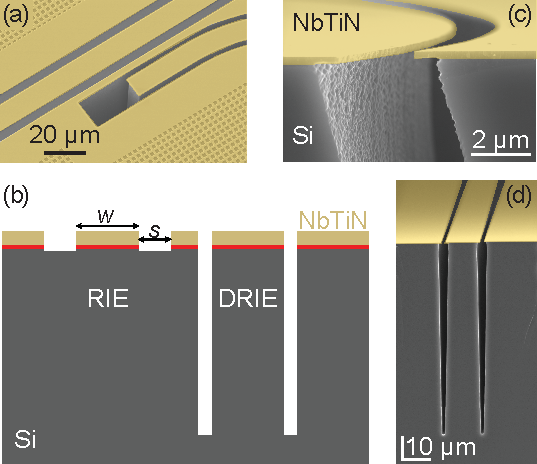
\includegraphics[width=.92\textwidth]{Figures/DRIE/DRIE figure.jpg}
    \caption{\textbf{(a)} false colored SEM image of a RIE feedline capacitively ocupled to a DRIE resonator. \textbf{(b)} Corresponding schematic cross-section. The metal substrate interface treated with HMDS is shown in red. \textbf{(c)} SEM cross section of a DRIE resonator near the surface, showing the metallization (\SI{\sim300}{\nano \meter}), Si underetch (\SI{\sim1}{\micro \meter}) and sidewall roughness (\SI{\sim100}{\micro \meter}). \textbf{(d)} SEM cross section of a DRIE resonator showing that a high etch anisotropy can be obtained, with a depth of \SI{80}{\micro \meter}.}
    \label{fig:DRIE schematic}
  \end{figure}

  \subsubsection{Magnetic shielding and vortex trapping}

  % \begin{wrapfigure}[20]{r}{0.4\textwidth}
  %   \begin{center}
  %   \vspace{-30pt}
  %     \includegraphics[width=\textwidth]{Figures/DRIE/Shielding.jpg}
  %   \end{center}
  %   \vspace{-20 pt}
  %   \caption{Different stages of shielding used. Inside the inner copper shielding is a black coating, used for IR absorption.}
  %   \label{fig:shielding}
  % \end{wrapfigure}
  Vortices are created in a superconducting thin film when a magnetic field greater than the sample-dependent threshold magnetic field is present. One method to lower the amount of vortices is to realize CPW with $w < \SIm{15}{\micro \meter}$, while using proper magnetic shielding around the sample. Furthermore, using nonmagnetic materials within the shield also result in less stray magnetic fields bring present.

  Even when using these methods to counter the presence of magnetic fields, there may still be a small amount of vortices present in the sample, which may lead to dissipation. To counter their movement a grid-like structure can be added in the superconducting material, effectively pinning the vortices.

  \begin{figure}[h]
    \centering
      \includegraphics[width=.4\textwidth]{Figures/DRIE/Shielding.jpg}
    \caption{Different stages of shielding used. Inside the inner copper shielding is a black coating, used for IR absorption.}
    \label{fig:shielding}
  \end{figure}

\chapter{Results and discussion}
\label{ch:Results and discussion}

  \section{Experimental set-up}
    \label{sec:Experimental set-up}


    \begin{figure}[!htb]
      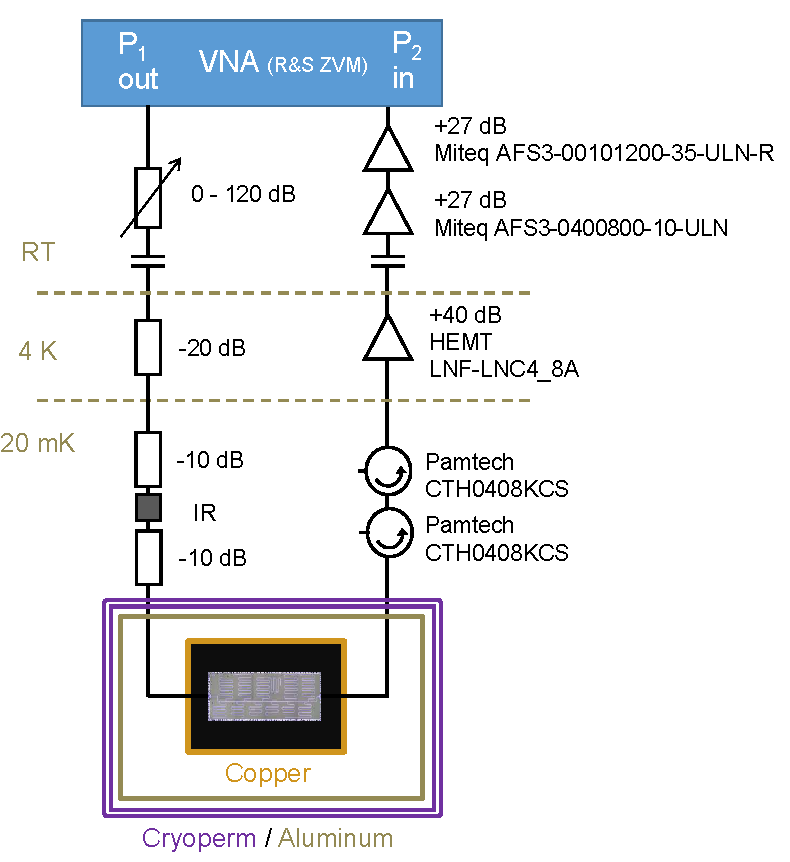
\includegraphics[width=.5\textwidth]{Figures/DRIE/FigS2_MW_setup.pdf}
      \caption[width=\textwidth]{Measurement setup used for resonator characterization in the $^{3}\mathrm{He}/^{4}\mathrm{He}$ dilution refrigerator (Leiden Cryogenics CS81): microwave schematic, magnetic shields (two Cryophy, one aluminum), IR filters (home-made Eccosorb filters), and IR adsorbers (inner surface of the inner Cu radiation shield, coated with Stycast~2850 and silicon carbide powder).}
      \label{fig:fridges}
    \end{figure}
    The experimental set-up is shown in Fig.~\ref{fig:fridges}. The fridge used in this experiment is a $^{3}\mathrm{He}/^{4}\mathrm{He}$ dilution refrigerator by Leiden Cryogenics. The refrigerator has a base temperature of \SI{\sim15}{\milli \kelvin}. Several stages of shielding are used. The sample is anchored to a copper coldfinger, directly connected to the mixing chamber of the dilution refrigerator. This is then enclosed in a copper can, the inner surface of which is coated in a mixture of Stycast 2850 and silicon carbide granules with diameters between 15 and 1000 nm to absorb IR radiation. The copper can is enclosed in a second can made from aluminum. The cans are furthermore surrounded by two layers of cryogenic magnetic shielding (1-mm-thick Cryophy, Magnetic Shields Ltd).

    The input signal is generated using a Rohde \& Schwarz ZVM vector network analyzer, connected to an Aeroflex 8310 step attenuator, which has an attenuation range of \SI{120}{\decibel}. The signal out of the fridge is measured using the same vector network analyzer.

    Using this set-up, quarter wave resonators, fabricated by Alessandro Bruno, were measured in a frequency range between \SIrange{1}{9}{\giga \hertz}. The sample is shown in Fig.~\ref{fig:set4}. The resonators were made using NbTiN on a silicon substrate. The advantage of NbTiN is that the metal atoms are bound to nitrogen, thereby inhibiting bond formation with oxides. In a way to minimize losses, all resonators were treated with HMDS and deep-reactive ion etching.


    Unless stated otherwise, all measurements were performed with the fridge at base temperature (\SI{\sim15}{\milli \kelvin}).

    Because the relevant regime where resonators interact with qubits is the single-photon regime, a very weak signal must must be applied to determine its properties in that regime. At these low powers noise becomes a relevant issue. In Appendix~\ref{ch:noise} the noise of the system is characterized.

    \begin{figure}[h]
      \centering
      \includegraphics[width=.7\textwidth]{Figures/DRIE/All_set4.png}
      \caption{Optical microscopy image of the sample measured for the APL paper. The sample consists of ten quarter wave resonators, with frequencies ranging between \SIrange{1}{11}{\giga \hertz}, connected to a central feedline. The resonators are made using NbTiN on a Si substrate. The sample is treated with HMDS and DRIE.}
        \label{fig:set4}
    \end{figure}



\section{Resonator measurement}

\begin{figure}[h]
    \centering
    \begin{subfigure}[b]{.49\textwidth}
        \label{fig:resonator_amplitude}
        \includegraphics[width=\textwidth]{Figures/DRIE/resonator_amplitude.png}\figureinset{(a)}{2.55}{2.0}
    \end{subfigure}
    \begin{subfigure}[b]{.49\textwidth}
        \label{fig:resonator_complex}
        \includegraphics[width=\textwidth]{Figures/DRIE/resonator_complex.png}\figureinset{(b)}{2.55}{2.0}
    \end{subfigure}
    \caption{Forward transmission $S_{21}$ spectrum of a resonator around \SI{2.75}{\giga \hertz}. Panel (a) shows the amplitude of $S_{21}$, along with a fit (red). Panel (b) shows the path of $S_{21}$ in the complex path, along with a fit (red). The green dot indicates the resonance frequency of the resonator.  Measurement was performed at \SI{15}{\milli \kelvin} at an input power of \SI{-123}{\dBm} corresponding to $\sim 5 \times 10^4$ photons.}
    \label{fig:resonator}
\end{figure}

 At or close to the resonance frequency, the resonator will interact strongly with the feed line, resulting in a reduction in transmission (see Fig.~\ref{fig:resonator}. The corresponding frequency spectrum exhibits a Lorentzian lineshape.

  In Fig.~\ref{fig:resonator} the transmission $S_{21}$ of a resonator is shown. Figure~\ref{fig:resonator}(a) shows the transmitted voltage $|S_{21}|$ of the resonator as a function of frequency. One interesting point is that the Lorentzian exhibits an asymmetry, which is often attributed to reflections in the feedline \cite[p192]{Geerlings}. This could be caused by impedance mismatching of components in the set-up, which would result in part of the signal being reflected.

  The data has in Fig.~\ref{fig:resonator} been fitted with the following complex-valued function~\cite{bruno2015reducing}:

  \begin{equation}
    S_{21} =A \left( 1 + \alpha \frac{\omega-\omega_r}{\omega_r} \right)
    \left(1-\frac{\frac{Q_l}{\lvert Q_e \rvert}e^{i\theta}}{1+2iQ_l\frac{\omega-\omega_r}{\omega_r}}\right)e^{i\left(\phi_v f+\phi_0\right)}.
    \label{eq:THEhanger}
  \end{equation}

  Here $\omega_r$ is the resonance frequency of the resonator, $Q_e=\left|Q_e\right|e^{i\theta}$ is the extrinsic quality factor, related to the coupling quality factor by $1/Q_c=Re\left(1/Q_e\right)$, $\alpha$ accounts for any slope in the background transmission surrounding the resonance frequency, and $\phi_v$ and $\phi_0$ account for the propagation delay to and from the sample.

\section{Power dependence}
\label{sec:resonator:results:power_dependence}

\begin{figure}
    \centering
    \includegraphics[width=0.8\textwidth]{Figures/DRIE/Qi_vs_n_photon.png}
    \caption{Internal quality factor of resonators as a function of mean number of photons present in the resonator. Measurements were performed at \SI{15}{\milli \kelvin}.}
    \label{fig:Qi_vs_n_photon}
\end{figure}
To be able to study the behaviour of the resonators, measurements were performed for several powers. Using proper calibrations for the attenuation down to the sample, the power can be converted to the input power at the sample. This value can then be converted to the mean number of photons present in the resonator, as described in Appendix~\ref{ch:photon number calculation}. The results are shown in Fig.~\ref{fig:Qi_vs_n_photon}.

As can be seen, all resonators measured obtain quality factors in excess of 1 million, even at the single photon regime used in quantum computation. It can furthermore be seen that the internal quality factor $Q_i$ of all resonators decrease with decreasing photon number. One explanation for this phenomenon is that the dissipation is mainly due to TLS. Since measurements were performed at \SI{\sim15}{mK}, the TLS are not saturated since the rate of thermal excitation is low. As discussed in section~\ref{sec:TLS}, the relative loss due to TLS is highest at low power, in the regime where they are not saturated. Therefore the fact that the internal quality factor $Q_i$ rises with the mean number of photons present in the resonator can be attributed to a larger amount of TLS being saturated. This would suggest that, even with HMDS and DRIE treatment of the sample, at low power and temperature, the internal quality factor is still limited by TLS being present.

As the mean photon number of a resonator is inversely proportional to the square of frequency \cite{bruno2015reducing}, for a low frequency resonator a lower input power is required to reach the same photon population as a higher frequency resonator. This has important consequences for the signal-to-noise ratio, and hence for the required integration time. At high photon numbers this is not a concern, as the transmitted signal is high enough to be accurately measured in a short period of time. For the single-photon powers, however, which is the region of interest for quantum computation, acquiring enough signal took up to five hours for the lowest frequencies. The reason that for the resonator with a resonance frequency at \SI{1.83}{\giga \hertz} has large error bars at low powers can be partly attributed to this, but as we will see in section \ref{sec:noise_results}, the main reason is that its frequency lies outside the bandwidth of the amplifiers and circulators of the set-up, resulting in a large amount of additional noise.

\section{Temperature dependence}
\label{sec:resonator:results:emperature_dependence}
\begin{figure}
    \centering
    \includegraphics[width=0.8\textwidth]{Figures/DRIE/Qi_vs_n_photon_temperature_dependence.png}
    \caption{Internal quality factor versus photon number for temperatures ranging from \SI{15}{\milli \kelvin} up to \SI{400}{\milli \kelvin}. All measurements were performed for a resonator with resonance frequency $f_0 = $\SI{2.75}{\giga \hertz}.}
    \label{fig:Qi_vs_n_photon_temperature_dependence}
\end{figure}

Aside from power, some of the dissipation channels also depend on the temperature of the system. To be able to study the effect of temperature on resonators, the resonator with frequency \SI{2.75}{\giga \hertz} has been studied as a function of power for several temperatures ranging from \SI{15}{\milli \kelvin} up to \SI{400}{\milli \kelvin}. The reason for choosing this resonator is that it has the highest internal quality factor of all the resonators measured, and so any change in quality factor would be most clearly visible.

The results are shown in Fig.~\ref{fig:Qi_vs_n_photon_temperature_dependence}. As can be clearly seen, the quality factor increases with increasing temperature. This is likely due to the fact that TLS are thermally excited for a larger percentage of time. Therefore, the relative energy dissipation with respect to total energy in the resonator will be lower, resulting in an increase in quality factor.

Another interesting point is that the increase in quality factor as a function of temperature is largest at low powers. This can also be explained when the limiting factor is due to TLS. At low powers, the TLS are almost exclusively excited thermally, while at higher powers, the excitation of TLS is not only due to thermal excitations, but also from photon absorption.

If one looks at the highest temperatures, it seems that the increase in quality factor as a function of temperature seems to slowly approach a saturation point. One reason is that the TLS are approaching their saturation, and so increasing the temperature further will have little effect on the percentage of time that the TLS are in the excited state. As will be shown in the next section, at \SI{400}{\milli \kelvin} the quality factor of the resonator is close to its maximum value, and will decrease as temperature is further increased.



\section{Temperature tracking}
\label{resonator:results:temperature_tracking}
\begin{figure}[h]
    \centering
    \begin{subfigure}[b]{.49\textwidth}
        \label{fig:temperature_tracking_Qi_drop}
        \includegraphics[width=\textwidth]{Figures/DRIE/Temperature tracking drop - Qi vs T.png}\figureinset{(a)}{2.65}{1.92}
    \end{subfigure}
    \begin{subfigure}[b]{.49\textwidth}
        \label{fig:temperature_tracking_Qi_nodrop}
        \includegraphics[width=\textwidth]{Figures/DRIE/Temperature tracking - no drop - Qi vs T.png}\figureinset{(b)}{2.57}{1.92}
    \end{subfigure}
    \caption{Internal quality factor versus temperature for the resonator with resonance frequency $f_0= $\SI{2.75}{\giga \hertz}. Quality factor was continuously measured as the sample was cooled down and warmed up four days later. Panel (a) shows the full temperature range up to the helium condensation cycle. Panel (b) shows a close-up of the region until \SI{900}{\milli \kelvin}.}
    \label{fig:temperature_tracking_Qi}
\end{figure}

To further investigate the temperature dependence of the resonator, a continuous measurement was performed on the resonator with resonance frequency \SI{2.75}{\giga \hertz} during a cool-down and a subsequent warm-up of the fridge four days later. Measurements were performed for temperatures ranging from base temperature (\SI{15}{\milli \kelvin}) to roughly \SI{1}{\kelvin}. Above this temperature, the fridge entered a cyclic helium condensation/evaporation process. All temperatures were measured at an input power of \SI{-113}{\dBm}, corresponding to roughly $5 \times 10^5$ photons. In Fig.~\ref{fig:temperature_tracking_Qi} the internal quality factor versus temperature is shown during a cooldown and subsequent warm-up of the fridge. As can be seen, the quality factor reaches a maximum quality factor at a temperature of \SI{\sim400}{\milli \kelvin}. Below this temperature, the quality factor is likely limited by the presence of TLS (see sections \ref{sec:resonator:results:power_dependence} and \ref{sec:resonator:results:emperature_dependence}). Above this temperature however, the quality factor decreases, indicating that TLS are not the limiting factor anymore for $Q_i$. One likely explanation is that the main source of dissipation is now due to the presence of quasiparticles in the resonator. At even higher powers other effects such as vortices contribute more significantly to the decay of the quality factor.

From Fig.~\ref{fig:temperature_tracking_Qi} it seems that there is some hysteresis at high temperatures. However, this is likely due to the fact that the thermometer is at a different position in the fridge as the sample, and does not thermalize equally fast. There may therefore be a delay between the temperature of the thermometer, and the actual temperature of the sample.

\begin{figure}[h!]
    \centering
    \includegraphics[width=.72\textwidth]{Figures/DRIE/Temperature tracking - f0 vs T.png}
    \caption{Resonance frequency versus temperature during a cooldown and subsequent warm-up four days later. In the period between cooldown and warm-up the resonance frequency has shifted by \SI{\sim 500}{\hertz}, possibly due to phase noise.}
    \label{fig:temperature_tracking_f0}
\end{figure}


Aside from the internal quality factor, another quantity of interest is the resonance frequency $f_0$ of the resonator, which also depends on the temperature. The result from of tracking the resonance frequency of the resonator during cooldown and subsequent warm-up is shown in Fig.~\ref{fig:temperature_tracking_f0}. As can be seen in both cases, the resonance frequency reaches a maximum around \SI{500}{\milli \kelvin}.

Between the cooldown and warm-up the resonance frequency seems to have shifted by roughly \SI{500}{Hz}. It is possible that during the four days that the sample was cooled the environment of the resonator slowly varied, which shifted the resonance frequency of the resonator. Further measurements are, however, required to determine if this is the case.

The decrease in resonance frequency at higher temperatures can be explained by the presence of quasiparticles, which increase the kinetic inductance \cite[p91]{Geerlings}. The resonance frequency is inversely proportional to the square root of the total conductance \cite{barends2008contribution}, and so an increase in kinetic inductance leads to a decrease in resonance frequency. For measurements done by Barends et al. \cite{barends2008contribution}, the change in resonance frequency due to changes in the kinetic inductance seem to roughly correspond with the decrease in center frequency measured in Fig.~\ref{fig:temperature_tracking_f0}.

\begin{figure}[h]
    \centering
    \includegraphics[width=.7\textwidth]{Figures/DRIE/Temperature increase tracking - f0 vs T with fit.png}
    \caption{Frequency shift versus temperature for low temperatures, along with fit (green). The fit was performed using the model by Gao et al.~\cite{gao2008experimental}. The fit corresponds well with data, even describing the frequency peak at the lowest temperatures.}
    \label{fig:f0_vs_T_with_fit}
\end{figure}

The decrease in resonance frequency at lower temperatures can be explained due to TLS still being present. A model is presented by Gao et al. \cite{gao2008experimental}, in which they describe the decrease in resonance frequency due to the presence of TLS. As can be seen in Fig.~\ref{fig:f0_vs_T_with_fit} the model corresponds well with the data at low temperatures. At higher temperatures the model deviates from data, which may be explained by quasiparticles dominating as source of dissipation. The model furthermore predicts an increase in resonance frequency at lowest temperatures, which Gao et al. have indeed measured~\cite{gao2008experimental}. This increase in resonance frequency can also be seen in Fig.~\ref{fig:f0_vs_T_with_fit}, further supporting the claim that at low temperatures the resonator is still limited by TLS, even after treatment of HMDS and DRIE.



\chapter{Conclusion and future work}

As we have shown, the application of HMDS surface treatment and DRIE resulted in an improvement of the internal quality factor of the resonators by almost an order of magnitude. These state of the art cQED CPW resonators all attained quality factors in excess of 1 million at single photon level, which is the regime at which cQED circuits operate.

Since the quality factor of all resonators is found to decrease with decreasing input power, this indicates that at low temperatures and powers the limiting factor is still due to TLS. The fact that the quality factor initially increases with higher temperatures, supports this claim. By also measuring  the resonance frequency as a function of temperature, the curve obtained is in good agreement with a model describing the resonance frequency shift due to TLS \cite{gao2008experimental}. The curve even shows an increase in resonance frequency at the lowest temperatures, which was also predicted by the model. These results suggest that even after HMDS surface treatment and deep-reactive ion etching was applied, the internal quality factor of the resonator at low temperatures and power is still limited by the presence of TLS. Further research needs to be done to determine at what interface the dissipation due to TLS is greatest.

The next step is to perform the same treatments (HMDS and DRIE) on transmon qubits, as it is expected that this will result in a similar increase in coherence times. This is, however beyond the task of my master thesis.



\part{Muxmon experiment}

  \textbf{large TODO:}
  \begin{itemize}
    \item Explain surface code architecture
    \item Explain the general structure of a chip:
    \begin{itemize}
      \item Feedline through which signal is sent and measured
      \item CPW resonators, capacitively coupled to feedline
      \item Single qubit coupled to resonators (coupling location?)
      \item Resonator buses
    \end{itemize}
  \end{itemize}

  \textbf{small TODO:}
  \begin{itemize}
    \item Rename DAC voltage to flux, and mention early on that this renaming will be used
    \item flux-bias line or flux bias line?
  \end{itemize}



  \chapter*{Introduction}

    At this moment circuit QED is at the stage where multi-qubit experiments are being realized.



  \chapter{Muxmon chip architecture}

    \textbf{Topics that should be explained in this section:}
    \begin{itemize}
      \item The Muxmon0 and Muxmon1 chip are designed with two purposes
      \begin{enumerate}
        \item Testing multiplexing using the Duplexer
        \item Explore qubit frequency re-use
      \end{enumerate}

      \item Explain similarities of chips
      \begin{itemize}
        \item Three qubits per chip
        \item All three qubits have individual flux tuning
        \item Air bridges are used, not only for connect the ground planes, but also such that the feed line can pass over other coplanar waveguides without contact \\
      \end{itemize}

      \item Explain differences between Muxmon0 and Muxmon1.
      \begin{itemize}
        \item The Muxmon0 chip has a driving line connected to each of the qubits. \\
            It has two resonator buses at \SI{4.9}{\giga \hertz} and \SI{5.0}{\giga \hertz}. \\
            These could also be used for two-qubit gates.
        \begin{description}
          \item[Advantage] Able to fully control each qubit individually, even when multiple qubits share the same frequency.
          \item[Advantage] Less coupling between data qubits.
          \item[Disadvantage] Requires more driving lines.
          \item[Disadvantage] Adds extra source of dissipation for the qubits.
        \end{description}
        \item The Muxmon1 chip has two driving lines, each capacitively coupled to one of the two data qubits, and to the ancilla qubit.
        \begin{description}
          \item[Advantage] Less driving lines required
          \item[Advantage] Less dissipation due to capacitive coupling
          \item[Disadvantage] Cannot individually control data qubit and ancilla qubit when they share the same frequency
          \item[Disadvantage] More coupling between qubits
        \end{description}
        \item Simplified model of the surface code
      \end{itemize}

      \item Explain concepts of cross-coupling and readout cross-talk
      \begin{description}
        \item[Cross-coupling] The coupling between qubits. \\
                    Cross-coupling leads to transfer of excitation.\\
                    An associated coupling strength \textbf{g} can be associated to cross-coupling.\\
                    Can be determined by driving one qubit extremely hard, and measuring signal from other qubit.\\
                    \textbf{TODO:} Show values of cross-coupling found, or do this in characterization section \\
                    \textbf{TODO:} Leads to coherent errors? \\
                    \textbf{TODO:} Two types of cross-coupling? Direct leakage of pulse pulse, and transfer of excitation? cross-driving?
        \item[Readout cross-talk] Coupling between a qubit and a resonator that are not directly coupled.\\
                      A part of the signal measured from one resonator is then due to the state of another qubit \\
                      \textbf{TODO:} Understand more behind readout cross-talk
      \end{description}

    \end{itemize}

    \textbf{Left to think about:}
    \begin{itemize}
      \item Should I already include items such as coherence times, the fact that Muxmon0 performs better than Muxmon 1?
      \item Where should I include coherence times versus frequency?
      \item Should the part on cross-coupling and readout cross-talk not be in characterization section?
      \item Should the section on the Duplexer go in here?
    \end{itemize}

    \textbf{Figures that need to be included:}
    \begin{itemize}
      \item Muxmon0 and Muxmon1 chip, preferably optical microscopy
      \item SEM image of air-bridges such that coplanar wave-guides cross without intersecting
      \item schematic of cross-coupling and readout cross-talk \\
          It could be good to create this using the actual Muxmon chip as background, with arrows indicating how the different effects operate
    \end{itemize}


  \chapter{Qubit characterization}
    \begin{description}
     \item[Description] This chapter gives a step-by-step description of how to find a resonator and qubit, and subsequently how to tune the qubit's parameters.
     \end{description}

    In the design of cQED chips, the parameters of the qubits and resonators are always targeted which are ideal for the experiment.
    For coplanar waveguide resonators one can already obtain relatively good parameters for the required dimensions from simple formulae \textbf{TODO:} refer to formula.
    For superconducting transmon qubits, however, finding the right dimensions that correspond to the desired parameters is a much more complicated process.
    The qubit's frequency, for instance, depends on the qubit's coupling energy $\Ec$ and Josephson energy $\Ej$. The coupling energy $\Ec$ can be reasonably estimated from classical simulations. Finding the right dimensions for the Josephson junction that result in the desired Josephson energy $\Ej$, however, is difficult, and usually physically testing different junctions is necessary to determine an accurate conversion from the desired $\Ej$ to the Josephson junction dimensions.

    Nevertheless, the actual parameters of the resonators and qubits are almost never where one expects them to be. Once the sample is cooled in the dilution refrigerator, an inevitable game of hide-and-seek follows with the goal of finding the frequency of the resonators and qubits, and subsequently determining their properties. This chapter describes the measurements that were performed to characterize the MuxMon samples.

    \section{Continuous-wave measurements}

      Once a sample is properly cooled down it is ready to be measured. At this stage the sample is still an unknown terrain, where the experimenter only has a rough map, containing the sample's targeted parameters, and the specific properties of the resonators and qubits.

      The first step is to look for signs of life. These manifest themselves as resonance frequencies of the resonators and the qubits that are coupled to them. As we are not yet interested in the properties of the resonators and qubits which can only be obtained through measurements with accurately timed pulses, we send continuous tones through the feedline, and measure deviations in the transmission. These measurements are known as continuous-wave measurements

      \subsection{Scanning for resonators}
      \label{sec:resonator-scan}
        Since communication with the qubits is mediated through their coupling to resonators, the first step is to find these resonators. This is done using a transmission measurement, in combination with heterodyne detection, and has been explained in section \textbf{TODO:} Create section in Resonator chapter.

        There is one difference in measuring a resonator when there is a qubit coupled to it. When considering the qubit as a two-level system, the behaviour of the coupled resonator-qubit system is governed by the Jaynes-Cummings Hamiltonian \cite{Reed}:

        \begin{equation}
          \hat{H} = \hbar \wres\left(\hat{a}^\dagger \hat{a} + \frac{1}{2} \right) + \frac{\hbar \wqub}{2}\hat{\sigma}_z + \hbar g \left(\hat{a}^\dagger \sigma_{-} + \hat{a}\sigma_{+}\right)
          \label{eq:Jaynes-Cummings}
        \end{equation}

        where $\wres$ is the bare resonance frequency of the resonator, $\wqub$ is the resonance frequency of the qubit's ground to excited state transition, and the qubit's two states are in the spin-representation. This Hamiltonian consists of three terms. The first term corresponds to the energy level of the resonator, the second to the energy level of the transmon, and the third is a coupling term between the two with coupling strength $g$.

        The difference between the resonator's frequency $\wres$ and the qubit's frequency $\wqub$ is given by the detuning $\Delta = \wqub - \wres$. If the magnitude of the detuning is large compared to the coupling strength $g$, the system is in the dispersive regime. In this case the Hamiltonian can be approximated by the dispersive Jaynes-Cummings Hamiltonian:

        \begin{equation}
          \hat{H} = \frac{\hbar \wqub^{'}}{2} \hat{\sigma}_z +  \left(\hbar \wres^{'} + \hbar \chi \hat{\sigma}_z\right) \hat{a}^\dagger \hat{a}
          \label{eq:dispersive-Jaynes-Cummings}
        \end{equation}

        The coupling between the qubit and resonator causes both qubit's frequency and the resonator's frequency to shift: $\wqub^{'} = \wqub + \chi_{01}$, $\wres^{'}=\wres - \chi_{12}/2$.

        Aside from experiencing a frequency shift dependent on the amount of detuning, Equation~\ref{eq:dispersive-Jaynes-Cummings} shows that the resonator also experiences a shift depending on the state of the qubit. The resonator's frequency is decreased by an amount $2 \chi$ when the qubit is in the excited state. The parameter $\chi$ is the dispersive shift, and is given by:

        \begin{equation}
          \chi = \chi_{01} - \chi_{12}/2 \approx \frac{g^2}{\Delta}\frac{\Ec}{\hbar \Delta - \Ec}
          \label{eq:dispersive-shift}
        \end{equation}

        where $\chi_{ij} = \frac{g_{ij}^2}{\omega_{ij}-\omega_c}$ are the partial dispersive shifts.

        Due to this coupling between resonator and qubit, it is important to choose the right RF power. When the amount of photons in the resonator reaches a certain point, this coupling will result in the resonator experiencing nonlinear effects. The resonator will thereby lose its Lorentzian lineshape. Therefore the RF power should be kept sufficiently low to avoid these nonlinear effects, while still maintaining a good signal-to-noise ratio.



        \textbf{TODO:}
        \begin{itemize}
          \item In the strong coupling regime (Leads to hybridization of qubit and resonator states: quton and fobit
          \item Explain that the quality factor is low because the resonator is coupled strongly to the qubit (equation including coupling to qubit?)
          \item Doesn't $\chi$ diverge when $\Delta \rightarrow \Ec$?
          \item explain concept of anharmonicity, and that $\alpha \approx E_c$
          \item Maybe explain concept of number splitting in dispersive Jaynes-Cummings. Number splitting is the phenomenon that the qubit's frequency shifts by an amount $2 \chi$ for every photon in the resonator.\\
                Alternatively mention this in another section.
          \item Mention that $g_{12}=\sqrt{g}$, and that other coupling strengths are exponentially suppressed in the transmon
        \end{itemize}

        \textbf{Figures:}
        \begin{itemize}
          \item Figure of transmission showing all three Muxmon0 resonators
        \end{itemize}

      \subsection{Powersweeping the resonators}
        Once the resonators have been located, the next stage is to find the qubit that is capacitively coupled to each of the resonators. Instead of directly scanning the entire frequency spectrum in search of the qubit, it is relatively straightforward to perform some initial measurements aimed at gaining information about our resonator and qubit, which will allow us to search for our qubit with much greater accuracy.

        As explained previously, the capacitive coupling between the resonator and qubit shifts the resonator frequency $\wres$ from its bare frequency. When the amount of photons in the resonator reaches a certain point, the resonator experiences nonlinearity, thereby losing its Lorentzian lineshape. When increasing the RF power even further, at a certain point the resonator regains its Lorentzian lineshape. In doing so its resonance frequency has shifted to its bare frequency $\wbare$. If this frequency shift is observed, it indicates that the resonator's frequency was shifted, and hence that the qubit is alive. Measuring this frequency shift is commonly done in a powersweep. A powersweep is a measurement in which a resonator scan is performed for a range of powers.

        A powersweep additionally provides information about at what power the resonator enters the nonlinear regime. For measurements involving the qubit the readout power must be below this threshold power. Furthermore, from the frequency shift between the dressed cavity frequency and the bare cavity frequency, the amount of detuning between the qubit and the resonator can be estimated using Equation~\ref{eq:dispersive-shift}.

        If no shift is observed, it could mean that the qubit is dead (e.g. because the Josephson junction is shorted). However, this is not necessarily the case. An alternative possibility is that the detuning between qubit and resonator is very large, and as a result the frequency shift cannot be discerned. At this point it is too early to draw conclusions, and we may almost draw the analogy with Schr\"odinger's cat in a box.

        \textbf{TODO:}
        \begin{itemize}
          \item Explain theory behind transition to bare cavity frequency (Reed's thesis has some information)
        \end{itemize}

        \textbf{Figures:}
        \begin{itemize}
          \item Powersweep of ancilla qubit
        \end{itemize}

      \subsection{Scan for qubit sweet-spots}
        Some of the qubits have a tunable resonance frequency. This is done through a superconducting quantum interference device (SQUID). In this case the two islands that compose the transmon qubit are connected by two Josephson junctions instead of one, effectively forming a loop. The SQUID loop is sensitive to the amount of flux passing through the loop. The amount of flux going through the SQUID loop can be changed by changing the surrounding magnetic field. This is commonly done by having a flux bias line in close proximity to the SQUID loop. Current flowing through the flux-bias line alters the magnetic field in the vicinity of the SQUID loop, and hence changes the amount of flux through the SQUID loop. A digital-to-analog converter is used to specify the amount of current that is sent through the flux bias line. Depending on the amount of flux through the SQUID loop, the resonance frequency of the qubit changes accordingly. these qubits are therefore called flux-tunable.

        For qubits that are flux-tunable, finding the sweet-spot of the qubit can be done without knowledge of the qubit's frequency. This can be done by sweeping the DAC voltage and measuring the shift in the resonance frequency. Because the frequency of the qubit varies as the amount of current through the flux-bias line changes, the detuning between the qubit and the resonator consequently changes. As a result the dispersive shift $\chi$, and therefore the resonator's frequency, also varies. At the sweet-spot of the qubit, the resonator's frequency $\wres$ is at a maximum. This is irrespective of whether the qubit's frequency $\wqub$ is above or below the resonator's frequency.

        The accurate way to measure the sweet-spot is to perform resonator scans as the DAC voltage is varied. The result is a 2D scan shown in \textbf{TODO:} Figure.

        A faster second approach for finding the qubit sweet-spot, at the cost of providing less information, is by choosing a fixed frequency close to the resonator's frequency $\wres$ (preferrably slightly below, where the transmission slope is steepest). By measuring the amount of transmission as the DAC voltage is being varied, one obtains essentially a line-cut of \textbf{TODO:} Figure. The idea this measurement is that if the qubit's frequency $\fqub$ decreases, the resonator's frequency also decreases, resulting in a decrease in transmission (closer to $\wres$). Likewise, if the qubit's frequency $\wqub$ increases, the resonator's frequency increases \textbf{TODO:} Why?, resulting in an increase in transmission (further away from $\wres$).

        At the qubit's sweet-spot, the resonator's frequency $\wres$ is at a maximum, and so the transmission should also be at a maximum. Furthermore, because the amount of detuning only depends on the deviation from the flux sweet-spot \textbf{TODO:} improve, the transmission should be symmetric with respect to the DAC voltage sweet-spot. If the resonator's frequency $\wres$ shifts by a large amount in the course of this measurement, it becomes harder to determine where the sweet-spot is (although even then often it can still be discerned). Nevertheless, this method is considerably faster than performing a full two-dimensional scan of frequency versus DAC voltage, and in most cases it works like a charm.

        In the case where the powersweep showed no measurable frequency shift, these two measurements are also useful in discerning whether or not the qubit is actually dead, or whether it was simply far detuned from the resonator.


        \textbf{TODO:}
        \begin{itemize}
          \item Explain how qubit's frequency has a cosine dependence on DAC
          \item Give detailed information on SQUID loop
          \begin{itemize}
            \item Why does the qubit frequency change in a SQUID loop
            \item Sweet-spot
          \end{itemize}
          \item Mention flux-noise?
          \begin{itemize}
            \item 1/f noise
            \item usually not limiting, as it is very slow
            \item This noise can be seen as occasional jumps (every few hours?) It would mean that every few hours the frequency must be recalibrated.
          \end{itemize}
        \end{itemize}

        \textbf{Figures:}
        \begin{itemize}
          \item SEM picture of SQUID loop, including flux-bias line
          \item Figure of 2D resonator scan vs DAC voltage
          \item Figure of 1D resonator fixed frequency DAC voltage scan
        \end{itemize}

      \subsection{Scanning for qubits}
        Once the preliminary measurements have been performed that characterize the resonators and provide hints about the whereabouts of the qubit it is time to actually find the qubit.

        The measurement to perform in order to find the qubit depends on the amount of detuning between the resonator and qubit, which can be estimated from powersweep measurements. If the amount of detuning is large compared to the coupling strength ($\Delta \gg  g$), the system is in the dispersive regime. In this case one commonly performs a two-tone spectroscopy to find the qubit's frequency. If, on the other hand, the detuning is comparable to the coupling strength ($\Delta \sim g$), the qubit and resonator are hybridized, and experience an avoided crossing. In such cases a normal transmission measurement suffices.

        If the qubit is flux-tunable, one important question to ask is: at what DAC voltage should the qubit be searched?

        One option is to choose zero DAC voltage. In most cases this is alright, but there are cases when this is a bad choice. For instance, trapped magnetic fields during cool-down could position the qubit near the anti-sweet-spot for zero DAC voltage, in which case finding the qubit will be next to impossible.

        A better option is to choose a DAC voltage that results in a detuning $\Delta$ that is large compared to coupling strength $g$, such that the system is in the disperisive regime. However, the detuning $\Delta$ should not be too high, as it would otherwise result in a negligible dispersive shift $\chi$.The optimum value is usually around a few hundred megahertz, although this is dependent on the device-specific parameters. The detuning can be approximated using powersweeps.

        \subsubsection{Spectroscopy}
          As was explained in section~\ref{sec:resonator-scan}, in the dispersive regime the resonator experiences a $2 \chi$ frequency shift dependent on the state of the qubit. In the case of a resonator capacitively coupled to the feedline, the transmission experiences a dip at the resonator's frequency. This dip will correspondingly shift when the qubit's state is switched. The transmission at the resonator's dip when the qubit is in the ground state will therefore be dependent on the state of the qubit (low when the qubit is in the ground state, high when the qubit is in the excited state). This is the property exploited in a two-tone spectroscopy measurement.

          In a two-tone spectroscopy measurement two tones are sent through the feedline.
          \begin{enumerate}
            \item A drive tone with varying frequency $\wdrive$.
            \item A measurement tone at the resonator's frequency when the qubit is in the ground state.
          \end{enumerate}

          The transmission through the feedline is measured while the frequency of the drive tone $\wdrive$ is swept. When the drive frequency $\wdrive$ is detuned from the qubit's frequency $\wqub$, the drive is off-resonant with respect to the qubit, and so we measure a low transmission due to a dip being present. However, when the drive frequency $\wdrive$ approaches the qubit's frequency $\wqub$, then the qubit will start to oscillate between its ground and excited state, with a rate dependent on the detuning between the drive frequency $\wdrive$ and the qubit's frequency $\wqub$. The qubit will therefore have a partial population in the excited state, resulting in a shift of the resonator frequency, dependent on the population in the excited state. This is measured as an increase in transmission.

          The minimum linewidth of the qubit using spectroscopy is set by its dephasing time $T^2$, which can be seen as the uncertainty in its frequency. However, the power of the drive tone causes an additional increase in the linewidth, due to stimulated emission of the qubit. This effect is known as power broadening. This effect can be quite useful for finding qubits, especially when designing high-quality qubits with a very narrow intrinsic linewidth. The optimal power for the drive strength is further dependent on the amount of detuning $\Delta$ between the qubit and resonator. The resonator effectively acts as a bandpass filter, centered around the resonator frequency. Therefore, the stronger the detuning, the more the drive tone is suppressed.

          The dispersive shift $2 \chi$ is also dependent on the amount of detuning $\Delta$ between the qubit and resonator. If the detuning $\Delta$ is large, the dispersive shift will be very small, and so the difference in transmission will also decrease. Since the resonator has a Lorentzian lineshape, at the resonance frequency this Lorentzian is flat, and so is insensitive to small deviations. To increase the contrast between the on-resonant and off-resonant transmission, it is usually advantageous to measure at a slight detuning $\delta$ away from the resonance frequency, where the transmission slope is high. Since the resonator frequency shifts down when the qubit is excited, it is better to have a positive detuning $\delta$ to ensure that the transmission increases as the drive frequence $\wdrive$ approaches the qubit frequency $\wqub$ and decreases as it leaves the qubit frequency.

          \textbf{TODO:} Spectroscopy section
          \begin{itemize}
              \item Is power broadening really due to stimulated emission?
              \item Explain optimal RF power
              \item Is the gradual increase really due to partial population? Is it then an average of the partial population? Or do you get other effects as well?
          \end{itemize}


        \subsubsection{Avoided crossing}
          When the detuning $\Delta$ between the qubit and resonator is not large compared to their coupling strength $g$, the qubit and resonator experience an avoided crossing. Because all of the qubits in the Muxmon chips are considerably lower in frequency compared to their resonators, the system is always in the dispersive regime, and so the system never approaches the avoided crossing. Nevertheless it is worth mentioning the avoided crossing briefly, as it is a breeding ground for interesting physics.

          At the avoided crossing the system is not in the dispersive regime, and so the dispersive Jaynes-Cummings Hamiltonian no longer applies. In this case the resonator and qubit are hybridized, and one can no longer speak of a qubit and resonator as separate entities. Instead, this hybridization results in a so-called quton and phobit.

          \textbf{Avoided crossing info:}
          \begin{itemize}
            \item The coupling strength $g$ is the minimum distance be~tween the splitting
            \item From Reed's thesis p.63 explanation of this avoided crossing is given\\
            \begin{align}
             E_0 = & -\frac{\hbar \Delta}{2}\\
             E_1 = & n \hbar\omega_r \pm \frac{\hbar}{2}\sqrt{4g^2n + \Delta^2}
            \end{align}\\
            Joining $E_0 + E_1$ results in a qubit approaching a resonator from the top.\\
            When the frequency of the qubit equals that of the resonator, the energy difference reaches a minimum, and is equal to $2g$.
          \end{itemize}

          \textbf{TODO:} Avoided crossing
          \begin{itemize}
            \item Explain the quton fobit behaviour near the avoided crossing
            \item Explain how one can extract coupling from avoided crossing
            \item Explain that for the Muxmon qubit this effect is not present
            \item Explain multiple lines near avoided crossing
          \end{itemize}

          \textbf{figures:}
          \begin{itemize}
            \item Figure of avoided crossing
          \end{itemize}


        \textbf{TODO:}
        \begin{itemize}
          \item Use relatively high source power, results in power broadening
          \item Mention what to do if qubit is close to or far away from resonator
          \item Mention the term transmission measurement earlier on.
          \item Pulsed spectroscopy
        \end{itemize}

      \subsection{Tracking the qubits}
        For flux-tunable qubits one is usually not interested in finding the frequency at one specific flux value. More important is finding how this frequency changes with varying flux. A naive approach would be to perform a two-dimensional scan of a fixed frequency range versus flux. At a certain flux the qubit crosses the boundary of the chosen frequency window. Every time this happens a new two-dimensional scan has to be performed with an updated frequency window. The larger the chosen frequency window, the less often this has to be updated. On the other hand, choosing a large window also means that a larger portion of the scan is spent not measuring the qubit. There is therefore a trade-off between measurement time and degree of human intervention. Furthermore, the resonator frequency also depends on the amount of detuning. Therefore the frequency of the measurement tone must also be updated every now and then.

        As an alternative approach I have created a modified version of the spectroscopy versus flux scan, known as tracked spectroscopy. In this approach after every spectroscopy scan the qubit frequency is extracted through fitting. From the qubit frequencies measured in previous scans the expected frequency at the next flux value is extrapolated. The frequency window of the next spectroscopy scan are then centered around the expected qubit frequency. The qubit is therefore tracked as its frequency changes. The same method is applied to update the resonator frequency.

        Tracked spectroscopy has several advantages over the two-dimensional spectroscopy versus flux scans. First of all, since the qubit's frequency follows a smooth curve (see Equation~\textbf{TODO:} Refer to eqn), the qubit's frequency can be estimated quite accurately. The frequency windows can therefore be narrow. This greatly reduces the measurement time. Secondly, tracked spectroscopy does not need any human intervention, as the frequency window is automatically updated after every spectroscopy scan. Therefore measuring the flux-dependence of the qubit frequencies is an automatized process (provided that the qubit frequency can correctly be extracted).

        For more information on the tracked spectroscopy algorithm see appendix~\ref{sec:Tracked spectroscopy}.

        \textbf{Improvements}
        \begin{itemize}
          \item Avoided crossing
          \item Variable RF and drive power
        \end{itemize}
        \textbf{TODO:}
        \begin{itemize}
          \item Maybe mention possible improvements
        \end{itemize}
        \textbf{Figures:}
        \begin{itemize}
          \item Tracked spectroscopy of qubit and resonator
        \end{itemize}

      \subsection{Flux matrix}
        When a current is passed through a flux-bias line, it is not only the flux through the SQUID of the qubit directly connected to it that is affected. Instead, the flux through SQUIDs of neighbouring qubits are also affected, albeit to a lesser extent. Therefore changing the frequency of one qubit by changing its corresponding flux-bias line current also affects the frequencies of the other flux-tunable qubits on the chip. The effect that the current passing through flux-bias lines has on the frequencies of the different qubits can be decoupled by correcting the flux cross-coupling effects. This is done by implementing a flux matrix.

        A flux matrix $\boldsymbol{F}$ is an $n \times n$ matrix, where $n$ is the number of flux-tunable qubits. Each row corresponds to a virtual flux, and can be interpreted as follows: in a row $F_i = \left[f_{i1}, \dots, f_{in}\right]$ each element $F_{ij}$ corresponds to the relative amount by which the flux-bias line of qubit $j$ should be changed, such that only the frequency of qubit $i$ changes, whilst the frequencies of the other qubits remain fixed. This results in $n$ decoupled virtual flux parameters.

        Creating a flux matrix is done by first determining for each qubit separately how much every flux-bias line affects its frequency. For a given qubit $i$ this can be found by tuning the qubit away from its sweet-spot using its main flux-bias line, to a point where the slope $\partial f_i/\partial V_i$ of the qubit frequency $f_i$ as a function of DAC voltage $V_i$ is steep. This is the region where we are sensitive to changes in qubit frequency. For the main flux-bias line we already know from tracked spectroscopy what the slope $\partial f_i / \partial V_i$ is at this point. For each of the remaining flux-bias lines we measure the slope $\partial f_i / \partial V_j$ as we vary the DAC voltage $V_j$ and measure the response of the qubit frequency $f_i$. The slope $\partial f_i / \partial V_j$ is a measure for the amount of flux cross-coupling, which should be considerably less than for the main flux-bias line. Finally dividing all the slopes by the slope $\partial f_i / \partial V_j$ of our main flux-bias line, results in the ratio's of the frequency response of qubit $i$ for each of the flux-bias lines. Performing this measurement for all the qubits results in a matrix $\boldsymbol{M}$, where each element $M_{ij}=\partial f_i / \partial V_j$ is the normalized frequency response of qubit $i$ when varying the DAC voltage of the flux-bias line corresponding to qubit $j$. The diagonal elements of matrix $\boldsymbol{M}$ should be equal to one.

        Tracked spectroscopy provides accurate information on the DAC voltage corresponding to the sweet-spot of a qubit. The sweet-spot may not lie exactly at zero DAC voltage. It may shift due to magnetic flux being trapped during the cooldown of the fridge. These sweet-spots are usually found in the case where all the remaining flux-bias lines are set to zero DAC voltage. There is a certain combination of DAC voltages $\vec{V}^{ss}$ for which all the qubits are at their simultaneous sweet-spot. This simultaneous sweet-spot can be found using matrix $\boldsymbol{M}$. We know for each qubit $i$ the DAC voltage $V^0_i$ corresponding to its sweet-spot. Since $\boldsymbol{M}$ stores the amount by which each flux-bias line affects the flux of any qubit, the qubit $i$ remains at its sweet-spot as long as $\boldsymbol{M}_i \vec{V}=V^0_i$ holds, where $\vec{V}$ is the vector containing the DAC voltages. Therefore the simultaneous sweet-spot $\vec{V}^{ss}$ can be found by solving the set of equations $\boldsymbol{M} \vec{V}^{ss} = \vec{V^0}$, where $\vec{V}^0$ contains the DAC voltages of the individual sweet-spots of the qubits.

        The flux matrix $\boldsymbol{F}$ can be found by inverting matrix $\boldsymbol{M}$. As mentioned earlier, each row of matrix $\boldsymbol{F}$ corresponds to the ratio by which the DAC voltages of the flux-bias lines need to be varied, such that the frequency of only one qubit is changed. We may therefore multiply each row by a different constant, as long as the ratio between the elements in each row stays constant. One can normalizing each row such that the main flux-bias line is equal to one. This has the advantage that there is a one-to-one correspondence between DAC voltage and flux, and as a result the tracked spectroscopy will look identical. Additionally, after the normalization each row can be multiplied by a factor such that the virtual flux is equal to the flux quanta present in the SQUID loop. This conversion factor can be obtained by fitting the qubit frequency curve obtained from tracked spectroscopy.

        For a given virtual flux vector $\vec{\Phi}=\left[ \phi_1, \dots \phi_n \right]$, the corresponding DAC voltages $\vec{V}$ are given by:

        \begin{equation}
          \vec{V} = \boldsymbol{F} \vec{\Phi} + \vec{V}^{ss}
        \end{equation}

        By adding the simultaneous sweet-spot DAC voltages $\vec{V}^{ss}$, we obtain the additional property that the sweet-spot of the virtual fluxes is set to zero.

        After determining the flux matrix $\boldsymbol{F}$, there will still be some small remaining cross-coupling, which depends on the accuracy of the measurements. The process of creating a flux matrix can then be repeated, but instead of using DAC voltages as the varying parameters to construct matrix $\boldsymbol{M}$, the virtual fluxes should be used. Furthermore, as the cross-coupling is small compared to before, the flux range can be much greater, such that small slopes can be accurately measured. The resulting flux matrix $\boldsymbol{F}_2$ can then simply be multiplied with the first flux matrix $\boldsymbol{F}$ to obtain a more accurate final flux matrix.






    \section{Time-domain measurements}
      \subsection{Qubit control}
        So far the measurements described have all dealt with continuous tones being applied and measuring the response in the transmission. These are crude measurements, that are nevertheless able to determine some properties of the qubit and resonator, such as their frequencies. However, to find more detailed properties of the qubits, such as their coherence times, one cannot apply a continuous tone, that drives some incoherent qubit population. Instead well-calibrated pulses are required, which modify the state of the qubit in a precise manner, corresponding to gates being applied to the qubit. These types of measurements are called time-domain measurements, as they require precise pulse timing.

        A simple time-domain measurement usually consists of two parts. The first part consists of controlling the qubit. Here pulses are sent which modify the state of the qubit. The second part consists of measuring the state of the qubit. This is done through a readout tone, similar to spectroscopy measurements. This readout tone projects the state of the qubit onto the Z-axis. From the response in the transmission the state of the qubit can be inferred. More complicated experiments may involve some sort of feedback loop, where additional qubit control can be applied depending on the measurement outcome. These measurements require the qubit readout to be quantum non-demolition, i.e. the state of the qubit is not destroyed in the process of qubit readout. This usually involves extremely low-noise amplification, such as through a Josephson parametric amplifier. Feedback measurements are not performed in this experiment, and are therefore beyond the scope of this thesis.

        Qubit pulses usually have a Gaussian shape. These pulses can be generated by modulating a carrier signal from an RF generator, and is commonly done using an Arbitrary Waveform Generator (AWG). For the Muxmon experiment the Tektronix AWG5014 is used, which has four channels, each of which can control its voltage output at the nanosecond scale. It further has eight marker channels, which can be used to trigger devices, such as RF generators and the Duplexer. The carrier signal is sent through the LO port of the mixer, and an AWG channel is connected to the IF port of the mixer. The ouput at the RF port of the mixer is the modulated signal, the amplitude of which depends on the amplitude of the AWG channel output.

        For IQ mixers it is also possible to modulate both quadratures of the carrier signal independently, using two AWG channels. This allows for single sideband modulation, which is done by convoluting the pulses of the I and Q quadrature channels with a sine and cosine respectively. The sideband modulation frequency $\omega_{sb}$ of these sinusoidal functions is the amount by which the carrier signal is shifted. Single sideband modulation has the advantage that the carrier frequency $\omega_c$ is shifted away from mixer leakage, which would otherwise cause a slight continuous rotation of the qubit. For more information on mixer leakage, see section~\ref{sec:Mixer calibration}.

        The length of the pulse is an important consideration. Shorter pulses allow for more qubit operations within its coherence time. On the other hand, the shorter a pulse is in time, the larger its frequency spectrum will be. At a certain point the spectrum will be so broad that there will be a nonnegligible signal at the qubit's excited-state to second excited-state transtion frequency. This will cause leakage to the second excited-state, thereby leaving the two-state Hilbert space.
        Furthermore, the finite resolution of the AWG causes the pulses to be discretized, resulting in the pulses being slightly distorted. The shorter the length of the pulse, the more discretization, and therefore distortion, will occur. This can cause further leakage to the second excited-state. It is therefore desirable to have a bandwidth, which is the inverse of the width $\sigma$ of the Gaussian pulse, that is small compared to the anharmonicity of the qubit.

        A second pulse, known as the Derivative Removal by Adiabatic Gate (DRAG) pulse \cite{motzoi2009simple}, can be applied along with the main pulse, to reduce the amount of leakage. The DRAG pulse is the derivative of the main Gaussian pulse, and adiabaticaly populates the second excited state during the pulse, and subsequently withdraws this population back to the two-state Hilbert space. Using the DRAG pulse can reduce the amount of leakage by orders of magnitude.

        \textbf{TODO:}
        \begin{itemize}
          \item Explain more on Z projection
          \item Explain more on non-demolition.
          \item Signal quadrature determines the rotation angle
          \item Mention that AWG channel amplitude must not be too high, and that attenuation should be used to avoid spurious resonant modes
          \item Refer to Noise chapter for more information on single sideband modulation?
          \item Mention that amount of rotation depends on time duration, refer to Reed's thesis
        \end{itemize}

        \textbf{Questions:}
        \begin{itemize}
          \item Are both quadratures modulated independently in IQ mixers?
          \item Why use sideband modulation?
          \item Why are Gaussian pulses used?
         \end{itemize}

         \textbf{Figures:}
         \begin{itemize}
            \item Gaussian pulse with derivative
          \end{itemize}

      \subsection{Calibrating drive amplitude}
        Performing gates on qubits requires knowledge of the parameters that define the pulse, such as the amplitude, phase, and pulse duration. The phase determines the axis along which the qubit is rotated. The duration and amplitude of the pulse determine the rotation angle. To rotate the qubit by a specific angle, either the pulse duration can be varied, keeping the amplitude fixed, or the pulse amplitude can be varied, keeping the pulse duration fixed. Both methods have advantages and disadvantages. Varying the pulse duration ensures that the maximum amplitude is roughly fixed, regardless of the rotation angle. On the other hand, pulses with a small rotation angle have a very small duration, and so their bandwidth will be large, which may lead to increased leakage. Varying the amplitude, on the other hand, ensures that pulses applied to multiple qubits end simultaneously, and so it is more natural to speak of a pulse clock cycle. In the measurements for this thesis the amplitude is varied, whilst the pulse duration is kept fixed.

        Determining the correct amplitude for qubit gates is commonly performed using a Rabi measurement. In this measurement the amplitude of a pulse with rotation along the X-axis is varied monotonically. The pulse will cause the qubit to rotate at a Rabi rate $\Omega_R$, which depends on the pulse amplitude.

        After application of a pulse with Rabi rate $\Omega_R$ and duration $\tau$, the wavefunction will be in state $\ket{\psi} = \cos{\left( \frac{\Omega_R}{2} \tau \right) } \ket{0} + \sin{\left( \frac{\Omega_R}{2} \tau \right)} \ket{1}$. After a measurement the qubit will be in the excited state with probability $\sin^2{\left( \frac{\Omega_R}{2} \tau \right)}$ \cite{Reed}. The Rabi rate $\Omega_R$ is proportional to the pulse amplitude.

        In a Rabi measurement the amplitude is swept monotonically from a negative value to a positive value. The result should look like a cosine, as shown in Figure \textbf{TODO}. The center of this cosine is where the amplitude is zero, and therefore corresponds to the ground-state of the qubit. At the other peaks, where the deviation from the ground-state is the largest, the qubit is in the excited-state. The amplitude of the left peak corresponds to a negative pi-pulse, and the right peak to a positive pi-pulse. Usually the amplitude step between successive segments is tuned such that the excited-state peaks are at specific segments.

        \textbf{Questions:}
        \begin{itemize}
          \item How does the rotation angle depend on the amplitude?
        \end{itemize}
        \textbf{TODO:}
        \begin{itemize}
          \item time variation or amplitude variation
          \item Refer to equation showing that rotation depends on time duration (Reed's thesis)
        \end{itemize}

      \subsection{Qubit decoherence}

        \subsubsection{Qubit relaxation}
          Once a pi-pulse has been tuned it is possible to excite the qubit. However, once the qubit is excited, it will not remain so indefinitely. Instead, the excitation will slowly leak away to different relaxation sources, some of which have been discussed in \ref{sec:Losses}. These sources of relaxation lead to an exponential decay of the qubit's excitation, with a relaxation time $T_1$. A typical measurement to characterize the relaxation time $T_1$ is performed by first applying a pi-pulse, and the waiting for a monotonically increasing wait time $\tau$, after which the state of the qubit is measured.

          relaxation time $T_1$,

          \begin{itemize}
            \item Purcell limit
          \end{itemize}


        \subsubsection{Qubit dephasing}
          Spectroscopy provides an estimate for the frequency of the qubit. However, even with pulsed spectroscopy, the accuracy is limited to roughly a megahertz. When the frequency of the driving tone $\omega_d$ is different from the qubit frequency $\omega_q$, the qubit will precess around the Z-axis with a frequency equal to the Rabi rate $\Omega_R = \omega_d - \omega_q$. This property is exploited in a Ramsey measurement, where the qubit frequency can be inferred from the precession rate. A Ramsey measurement is performed by first applying a $X_{\pi/2}$ pulse, after which the qubit lies on the equator of the Bloch sphere. The state of the qubit then starts to precess around the equator, with a rate determined by the amount of detuning $\Delta$. After a certain wait time $\tau$, an $X_{-\pi/2}$ pulse is applied to the qubit.

          At the moment we ignore effects such as decoherence and gate errors. If there were no precession, the qubit should be pulsed back exactly to its ground state. However, any detuning $\Delta$ causes the state of the qubit to deviate from its original position on the Bloch sphere, and so the second pulse does not exactly cancel the effect of the first pulse. in fact, after half a period the second pulse results in the qubit being in the excited state. After one full period, however, the qubit has returned to its original position on the equator, and so the second pulse will yet again return the qubit to the ground state. In a Ramsey measurement the final state of the qubit is measured as the wait time $\tau$ between the two pulses is monotonically increased. The result should exhibit an oscillatory behaviour, the frequency of which being equal to the Rabi rate $\Omega_R$.

          In reality however, the qubit does suffer from decoherence. Especially phase noise, characterized by the dephasing time $T_2^*$, is noticeable in a Ramsey measurement. Phase noise can be seen as fluctuations in the qubit frequency. The dephasing time $T_2^*$ has an upper bound equal to $2\;T_1$, but can decrease significantly due to other sources of phase noise, such as charge noise, fluctuating cavity photon number, and flux noise for flux-tunable qubits \cite[p.~126]{Sears}. The result of dephasing is that the oscillations will decrease in amplitude as the wait time is increased. For a Ramsey measurement the excited-state population $P_1$ as a function of wait time is given by:

          \begin{equation}
            P_1(t) = e^{t/T_2^*} * \cos{\left( 2 \, \pi \, \Omega_R \, t \right) + 1/2}
            \label{eq:Ramsey}
          \end{equation}

          Usually in a Ramsey measurement artificial detunining is added to the pulse, such that if there were no real detuning, one would see around three to four oscillations. There are several reasons for this artificial detuning. One reason is that estimating the detuning using Equation~\ref{eq:Ramsey} is more accurate once there are several oscillations present. Another reason is that if the real detuning is reasonably small compared to the artificial detuning, it is possible to estimate if the qubit's frequency is higher or lower than the drive, as this would result in a higher or lower oscillation frequency.



          \begin{itemize}
            \item coherence time, drive amplitude
            \item Accuracy of calibrating the frequency depends on the dephasing time $T_2^*$
            \item Two $T_2^*$ values, one for exponential? noise, one for Gaussian noise
            \item dephasing is maximum twice relaxation
          \end{itemize}

          \textbf{Questions:}
          \begin{itemize}
            \item How is the Rabi rate $\Omega_R$ related to the detuning?
            \item Where does exponential noise and Gaussian noise come from? As I understand it Gaussian noise is due to flux
            \item Is $T_1$ not noticeable in a Ramsey measurement?
            \item Dephasing results in a mixed state, and therefore shrinks towards the Z-axis on the Bloch sphere?
          \end{itemize}

          \textbf{TODO:}
          \begin{itemize}
            \item Remove parts about frequency tuning, add that in calibration section
          \end{itemize}

          \textbf{Figures:}
          \begin{itemize}
            \item Ramsey measurement
            \item $T_2^*$ vs. frequency?
          \end{itemize}

        \subsubsection{Echo measurement}

          \begin{itemize}
            \item Refocusing
          \end{itemize}


      \subsection{Motzoi parameter}
      \subsection{AllXY measurement}
      \subsection{Measuring single shots}




  * [ ]Explanation of gates
  * [ ]Motzoi parameter
  * [ ]Calibrating drive amplitude using Rabi
  * [ ]Calibrating frequency using Ramsey
  *
    * Conflict with next section on accurate tune-up?

  * [ ]Measuring decoherence
  *
    * Relaxation
    *
      * T1 measurement

    * Dephasing
    *
      * Ramsey measurement (all noise)
      * Echo measurement (fast noise)

    * Change with frequency
    *
      * Ideally T2 is 2*T1
      * T2 rapidly decreases as moving away from sweet-spot


  * [ ]Single-shot measurements
  *
    * Able to see relaxation and thermal excitation

  * [ ]Second excited state
  *
    * Similar to three-tone spectroscopy
    * Nearly identical position in IQ-plane as first excited state, but less relaxation into ground state
    * Since time-trace is averaged, the final signal is therefore further away from the ground state in the IQ-plane

  * [ ]Crosstalk / cross-coupling?




  \chapter{Calibration routines}
    \section{Accurate frequency estimation}
    \section{Mixer calibration}
      \label{sec:Mixer calibration}

  \chapter{Randomized benchmarking}

    \section{Second excited state}

\begin{appendices}

\input{Chapters/appendix.tex}

\end{appendices}

\bibliographystyle{plain}
\bibliography{bibliography}


\end{document}